%Big Bounding box around, no quadtree used

Wenn die Element zu dicht beieinander oder sogar aufeinander bzw.überdeckend sind, kann es sind, dass der Quadtree ineffizient wird.
Dies ist vor allem der Fall, wenn man weit rauszoomt.
Dann ist der Graph quasi auf einem Punkt und um ihn herum ist viel ungenutzter Raum.

Ob der Zoom Mode nutzbar ist, wird kontrolliert, wenn der Quadtree sich als ineffizient deklariert.
Hierfür werden von allen Knoten minimalen und maximalen $x$- und $y$ Werte ermittelt und
aus diesen eine große Bounding Box generiert, die dann den Graph vollständig enthält.

Diese Bounding Box des Graphen wird mit den Bounds verglichen und es wird überprüft, ob
oberhalb oder unterhalb der Graph-Bounding Box noch wenigstens eine Labelhöhe Platz ist oder
ob sich links oder rechts davon noch wenigstens eine Labelbreite ungenutzter Raum befindet.

Findet sich an wenigstens einer Seite solch ungenutzter Raum, dann wird mittels \hyperref[subsubsec:spiral]{Spiral Model} versucht, eine Position in diesem Raum zu finden.
Wird eine solche Position gefunden, ist sie in-bounds und hat keine Überdeckung mit der Bounding-Box des Graphen.

Spiral Model wird verwendet, da dies der einzige Algorithmus ist, der sich inkrementweise von seinem Ursprung (also dem korrespondieren Knoten) entfernt und man mit der Position des Labels
außerhalb der großen Bounding Box des Graphen landen muss.
Die wäre mit den anderen Algorithmen nicht zuverlässig möglich.
Wie bei Spiral Model üblich werden die tatsächlichen Labels mit einer Hilfslinie zum Knoten verbunden.

Tatsächliche Labels werden hier nicht in den Quadtree einsortiert, da er im Zoom Mode nicht genutzt wird. Stattdessen werden sie sich direkt gemerkt.
Der Performancegewinn hier ist, dass alle Knoten als eine Bounding Box dargestellt werden, und man somit im Prinzip nur Labelpositionen miteinander, aber nicht mit Knoten vergleichen muss.

In der Praxis ist die Anzahl der gelabelten Knoten konstant (siehe \hyperref[subsec:consts]{Magic Constants}) und nur ein Bruchteil der zu sehenden Knoten,
sodass die quadratische Komplexität hier noch nicht zu Performanceeinbußen führt.

Kantenlabeling findet im Zoom-Mode nicht statt, da die Kanten praktisch von den Knoten im Zoom überdeckt werden und hier auch Berechnungen eingespart werden können.

\begin{figure}[H]
    \centering
    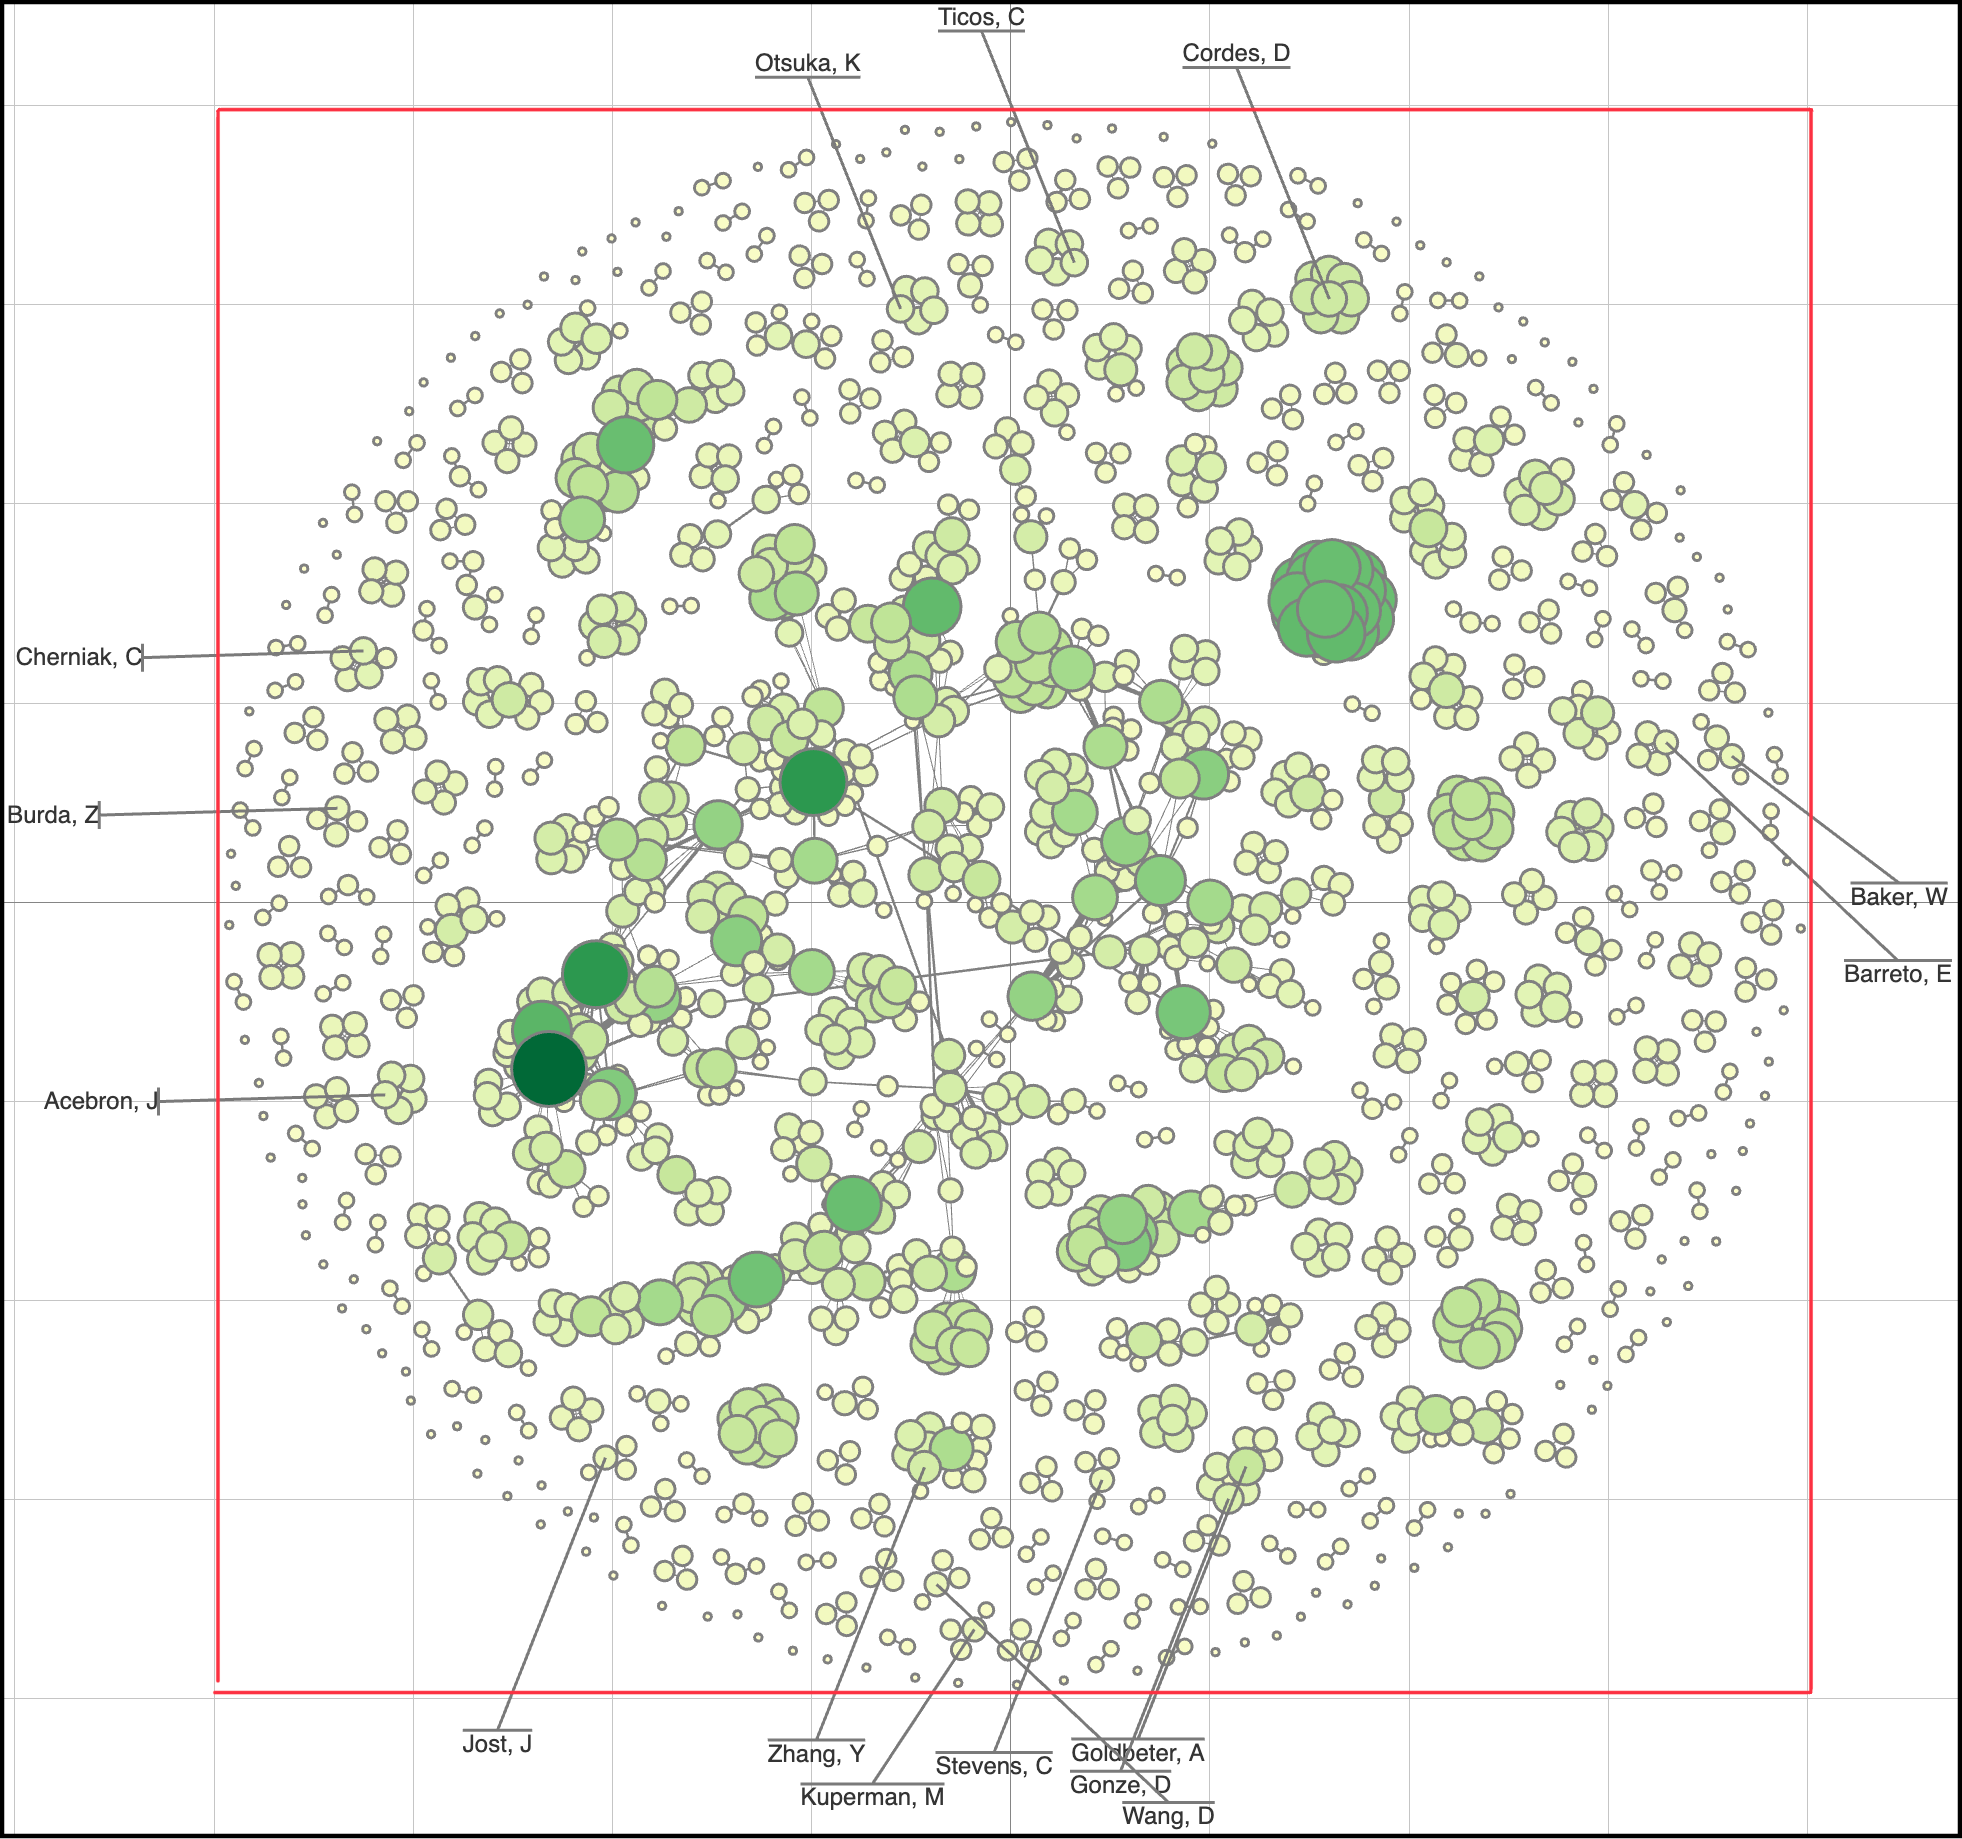
\includegraphics[scale=0.14]{../img/zoom}
    \caption{Zoom Mode aktiv. Außerdem zu sehen: Hilfslinie zwischen Knoten und Labels}
    \label{fig:zoom}
\end{figure}